% !TEX root = ANA-GENR-2018-01-INT1.tex
% Turn off some chktex warnings.
% chktex-file 1 chktex-file 8 chktex-file 46

%------------------------------------------------------------------------------
\section{FENCE and GitLab integration}%
\label{sec:FENCE_and_Gitlab_integration}
%------------------------------------------------------------------------------

As mentioned in section \cref{sec:Analysis_and_paper_phases}, the FENCE Analysis/Phase 0 system was designed and implemented in order to provide an automatic creation of Git repositories for each Analysis or publication. So the Phase 0 functionalities encompasses some features that triggers the GitLab commands. The integration between the software framework and the collaborative repository  platform will be described in details in this section.

%------------------------------------------------------------------------------
\subsection{GitLab structure to organise analysis groups and repositories}%
\label{sec:Gitlab_structure_to_organise_Analysis_groups_and_repositories}

Analysis groups and repositories are created in GitLab under the atlas-physics-office group. Each leading Physics, Combined Performance group or a System Detector/Activity coordination is labelled as a category with four letters in FENCE Analysis systems.

\begin{table}[h]
\centering
\begin{tabular}{ll}
BPHY & B physics WG                 \\
EGAM & e/gamma CP                   \\
EXOT & Exotics WG                   \\
FTAG & Flavour tag CP               \\
HDBS & Higgs \& Diboson Searches WG \\
HIGG & Higgs WG                     \\
HION & Heavy Ions WG                \\
IDTR & Inner Detector Tracking CP   \\
JETM & Jet/Etmiss CP                \\
MUON & Muon CP                      \\
PMGR & Physics Modelling Group      \\
SIMU & Simulation                   \\
STAT & Statistics Committee         \\
STDM & Standard Model WG            \\
SUSY & SUSY WG                      \\
TAUP & Tau CP                       \\
TOPQ & Top WG                       \\
UPPH & Upgrade Physics             
\end{tabular}
\caption{List of Leading Groups and description }
\label{tab:my-table}
\end{table}


For example, the leading Top Quark physics group is \texttt{TOPQ} while the Electron/Gamma Combined Performance group is \texttt{EGAM}.
The ID of a Phase 0 FENCE entry is therefore labelled: \texttt{ANA-GROUP-YEAR-NN} where GROUP can be \texttt{TOPQ}, \texttt{HIGG} or \texttt{EGAM}, for example.
\texttt{YEAR} is the year when the document was created and \texttt{NN} is a two digit number.
For instance, ANA-SUSY-2019-04 for the 4th Analysis FENCE entry created in the SUSY group in 2019.

An analysis group may evolve into a Paper, a CONF or a PUB note. The IDs of those documents are therefore respectively \texttt{GROUP-YEAR-NN}, \texttt{CONF-GROUP-YEAR-NN} or \texttt{PUB-GROUP-YEAR-NN}.
This naming convention preserves the backward compatibility with the different entries used for each type of document before Phase 0 creation.

In PO-Gitlab, an effort has been made to make the document IDs  more logical.
They are labelled: \texttt{ANA-GROUP-YEAR-NN-INTn} for an internal note,
\texttt{ANA-GROUP-YEAR-NN-PAPER} for a paper,
\texttt{ANA-GROUP-YEAR-NN-CONF} for a CONF note,
\texttt{ANA-GROUP-YEAR-NN-PUB} for a PUB note.
For example, in the Higgs category, for a given Phase 0 Analysis entry \texttt{ANA-HIGG-2017-08},
\pogitlab will host \texttt{ANA-HIGG-2017-08-INT1,2..n, ANA-HIGG-2017-08-PAPER, ANA-HIGG-2017-08-CONF, ANA-HIGG-2017-08-PUB}.
Each repository is connected to the appropriate FENCE interface.
This can be seen in \cref{fig:Gitlab_repository} where the \gitlab interface for the atlas-physics-office subgroups and repositories is shown.
\texttt{ANA-HIGG-2017-08}, a subgroup of HIGG, in fact contains one paper and one internal note repository, namely \texttt{ANA-HIGG-2017-08-PAPER} and \texttt{ANA-HIGG-2017-08-INT1}.

\begin{figure}[htb]
  \centering
  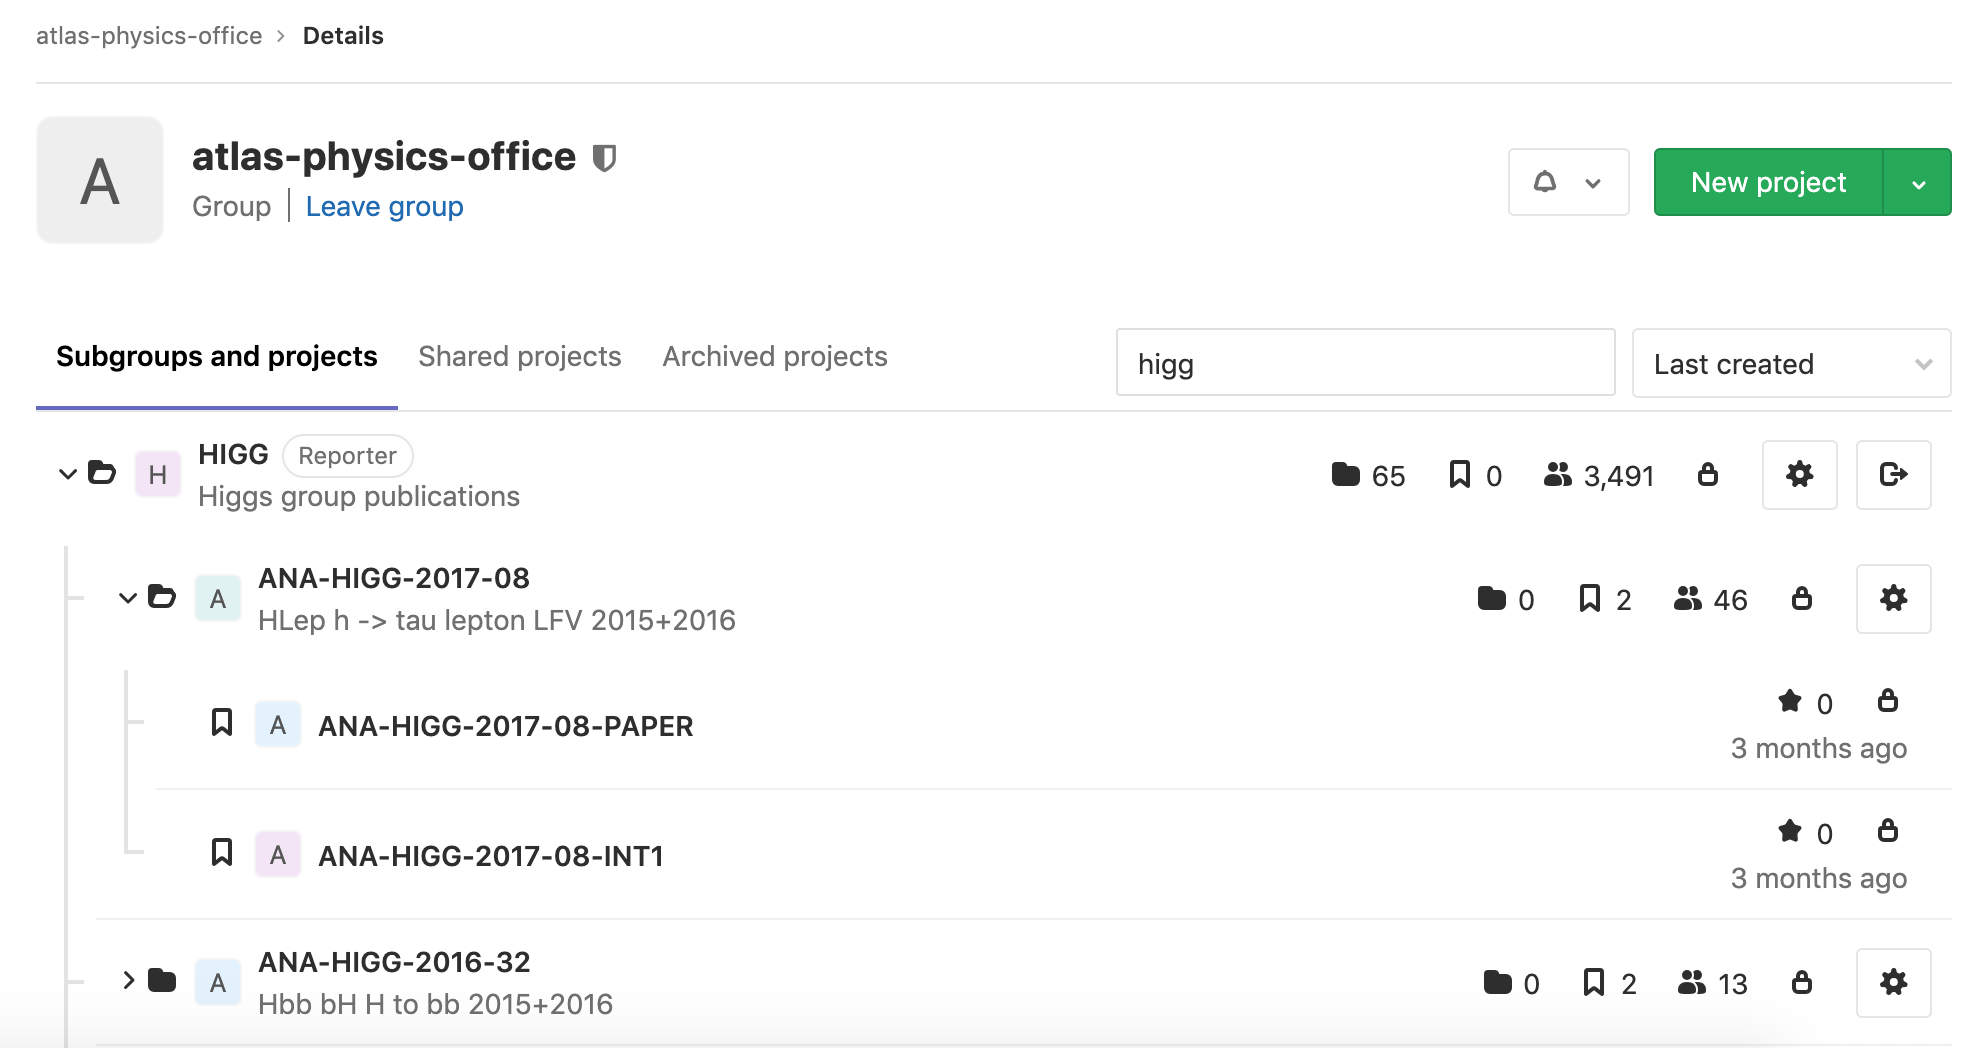
\includegraphics[width=0.9\textwidth]{Gitlab_repository}
  \caption{Screenshot of the substructure of a HIGG Gitlab repository. The main group atlas-physics-office is shown on the top. The HIGG subgroup is selected, and its ANA-HIGG-2017-08 subgroup is expanded. A repository for the PAPER, and one for the Internal Note number 1 are created under ANA-HIGG-2017-08}%
  \label{fig:Gitlab_repository}
\end{figure}

%------------------------------------------------------------------------------
\subsection{Middleware between FENCE and Gitlab REST API}%
\label{sec:Middleware_between_FENCE_and_Gitlab_REST_API}

A set of classes were created with the original aim of making the usage of the \gitlab API easier between the FENCE systems.
In fact, it is mostly used by the Analysis systems within the Analysis Gitlab integration.
Through the main class, called \Class{Gitlab}, it is possible to handle all the basic operations offered by the API\@: create, get and customise settings for projects, groups, branches, handle commits and many other actions defined and explained in the Gitlab REST API documentation~\cite{rest_api}.

Each API endpoint can be accessed by one of the following HTTP methods: GET, POST, DELETE and PUT\@.
The FENCE--\gitlab class uses them through methods detailed in \cref{app:fence:gitlab:methods}.
Each of those methods make a call to \Class{execMethod}, in \cref{app:fence:gitlab:execmethod},
that configures the endpoint using the PHP CURL methods~\cite{php_curl} and executes one of the HTTP methods, returning the REST API answer, that can be a JSON file with metadata, or just a success, or an error message.

The metadata returned by the \Class{execMethod} is then used to populate the attributes of many classes representing some \gitlab elements like:
\texttt{Branch, File, Commit, Project, Group, Label} and \texttt{Member}.
These can be then manipulated by any FENCE system.

An example is the creation of a paper repository.
The \Class{createProject} method (see \cref{app:fence:gitlab:createproject}) is called having the project name as the first argument
(or even an instance of the \Class{Project} class) and project parameters as the second argument like path, namespace, default branch, description and others.
The method calls the POST method mentioned above and stores the new repository metadata in a FENCE \Class{Project} object, which can be used for further manipulations.

\GSnote{}{Example code snippet here???}


%------------------------------------------------------------------------------
\subsection{FENCE-Gitlab Integration}%
\label{sec:FENCE-Gitlab_Integration}
The first interaction between FENCE and \gitlab happens when a Phase 0 entry is created.
A group with its reference code is automatically formed containing the first internal note repository.
The content of this repository’s first commit is obtained from a source repository,
which is the package containing file templates called \texttt{atlaslatex}.
FENCE is responsible of substituting all the necessary variables in all the file templates according to the metadata inserted when creating the entry in the system. After the commit, FENCE automatically un-protects the master branch, creates the protected PO-ready branch and also creates PO-Publication label. The last step is to set the developer permission to the Analysis Team egroup using LDAP synchronisation.

Another FENCE and \gitlab integration process is executed when Phase 0 is finished or is skipped, proceeding to Paper, CONF or PUB note Phase 1.
FENCE automatically creates an internal note repository setting all the configuration needed.
It is also possible to append one or more additional internal note repositories at any time.
The creation of the configuration of the repositories holding the document is done without any input from the editor’s side, allowing for a quick process.

FENCE and Gitlab also interact while handling the author list of a publication.
Creating the author list at first circulation will trigger a request for the existence of the \gitlab repository associated to the publication through the Gitlab API\@.
In the transition period from the old to the current system,
if the repository did not exist, the author list would have been stored on a volume under the Andrew distribuited File System (AFS) directly accessible, for instance, through a terminal session.
The old system is now deprecated.
Nowadays a \gitlab repository associated to the paper is a mandatory prerequisite, and to force the user to use it,
FENCE will not allow the creation of the author list until the repository, if missing, is created.

The act of clicking on the button labeled as \enquote{Create and push to Gitlab}, see \cref{fig:paper_authorlist_section}, creates the author list according to its reference date in all the different formats (\File{xml}, \File{tex} and others).
It then starts a dialog among the two platforms, FENCE and \gitlab, to correctly push the files through the \gitlab API.
On first circulation, the files are added to \gitlab, while on following circulations, as they already exist, they are simply updated.

\begin{figure}[htb]
  \centering
  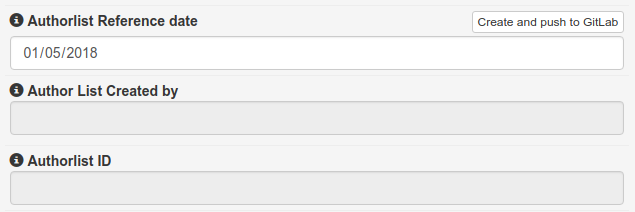
\includegraphics[width=0.9\textwidth]{paper_authorlist_section}
  \caption{A view of a paper's author list section: on first circulation,
  the \enquote{Create and push to GitLab} button generates the author list and triggers the push action on the GitLab repository.
  The button will change its label on following phases to \enquote{Generate and push to GitLab}.}%
  \label{fig:paper_authorlist_section}
\end{figure}

Another level of interaction is needed to avoid an error that will result in a blocker operation.
Through the \gitlab API we can, as said, upload a new file, or update an older one, using two different methods, \Class{add} and \Class{update}.
Trying to add a file that already exists or to update a file that doesn't exist will result in a blocker operation, so we always need to verify which is the correct operation that applies.
It might seem redundant as a check, because on first circulation the files are never expected to be there, and from second circulation we always know the file must already be there. But the repository can be accessed in many ways and the users can, by mistake, move, rename, delete, add files by their own. If any of these cases occurs, we need to be sure to be able to handle the situation without generating further errors.
